
\section{Implementation}


The project implements the following pipeline (see figure \ref{core2js}):
\begin{enumerate}
\item Serialize Haskell program: 
  \begin{enumerate}
  \item Create external-core file from Haskell program using GHC.
  \item Create JSCore from external-core using the extcore and JSON packages.
  \end{enumerate}
\item Deserialize JSCore:
  \begin{enumerate}
  \item Parse JSCore using the parsing tools available for PyPy
  \item Build Core AST from resulting JSON datatype
  \end{enumerate}
\item Evaluate program:
  \begin{enumerate}
  \item Evaluation is done by the already implemented PyPy Core' interpreter,
  Haskell-Python. Additional functionality had to be built on top of this, mostly 
  Haskell library functions.
  \end {enumerate}
\end{enumerate}

\subsection{Tools and versions}

The following tools and package versions was used in the implementation:

\begin{itemize}
\item GHC version 7.0.3
\item extcore version 1.0.1
\item PyPy current head branch (Last tested 09/11/2011)
\item Haskell-Python interpreter: Interpreter of core written in RPython
\item Python 2.7: Used to test the Core' interpreter without it having to be correct RPython.
\end{itemize}

%\paragraph{GHC} version 7.0.3. Binary version. % Source needed for creating extcore with correct grammar file.

%\paragraph{genprimopcode} --make-ext-core-source < \{path/to/primops.txt\} > \{path/to/PrimEnv.hs\}

%\paragraph{extcore} version 1.0.1, %Source version, updated with grammar of external-core for GHC version 7.0.3 (See extcore 1.0.1 README file for details)

%\paragraph{PYPY} current head brach.

%\paragraph{Haskell-Python} interpreter of core written in RPython.

\subsection{Organization}

The implementation is organized as represented by figure \ref{organization}. The
main folder (interpreter) contains the main program, and a program for generating
dot files, "makegraph.py" (used to create graphs of parsed JSCore files using graphviz). 
The "haskell" folder
contains the PyPy Core' interpreter code, used by the main program for evaluation, 
and by the parser to generate the abstract-syntax-tree (AST). In addition to this,
the subfolder packages implements some simple functionality to used by the test-programs.
Among others, a very simple IO function for printing text to the terminal (putStrLn).
These packages are loaded and references to the functions they contain are used during
the creation of the AST. See figure \ref{core2js} for a brief description of the pipeline.

The "core" folder contains Haskell program for generating JSCore files from external-core
files, the JSCore parser, and a simple datastructure representing Haskell modules.

\begin{figure}[H]
\centering
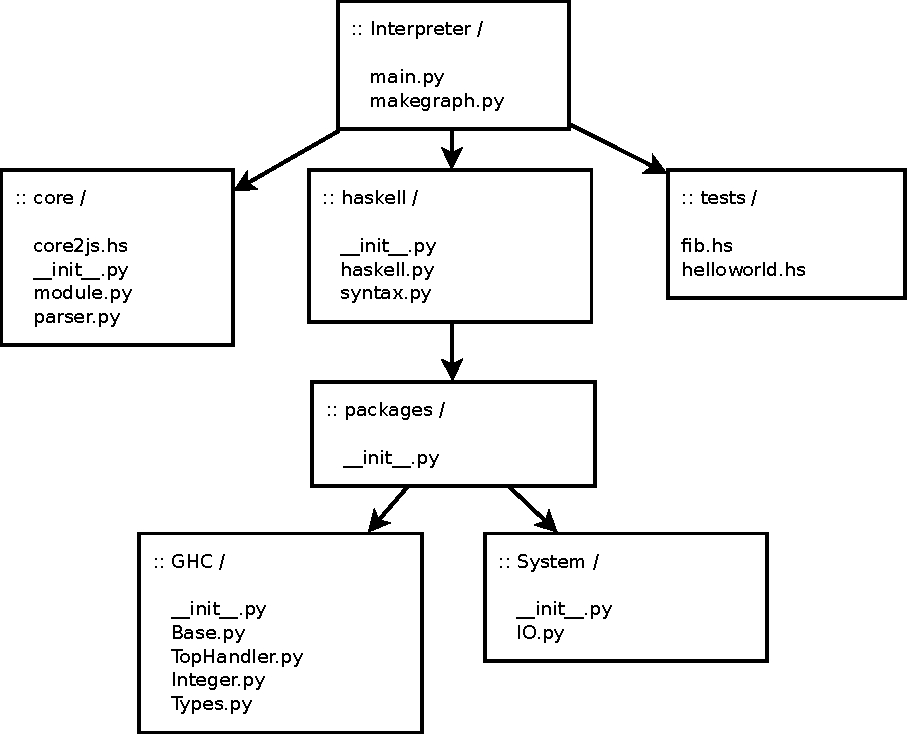
\includegraphics[width=0.8\textwidth]{diags/organization}
\caption{Code tree: The top of the boxes is the folder name, and the rest is the source 
files. Arrows represent subfolders.}
\label{organization}
\end{figure}

\subsection{Serializer}

The serializer consists of two parts; GHC generating external-core, and 
a Haskell program to generate JSCore.

External-core is easily generated by using a compiler flag:
\begin{lstlisting}
ghc -fext-core {path-to-program}
\end{lstlisting}

\begin{figure}[H]
\centering
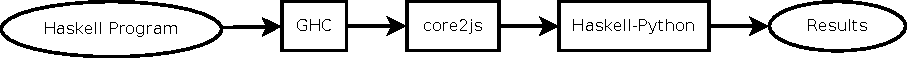
\includegraphics[width=0.8\textwidth]{diags/pipe_w_core2js}
\caption{Pipeline implementation with core2js using extcore}
\label{core2js}
\end{figure}

The Haskell program generating JSCore uses the extcore packages. This package
implements functionality for working with external-core. The result is a datastructure
mapping directly to the external-core format defined in \cite{tolmach2010ghc}. By traversing
this structure, the program builds up a JSON tree using the Haskell JSON package.
The result is a tree of JSON constructs (corresponding to the grammar defined in table \ref{jscore}), 
this is then pretty-printed and dumped to a file.

\subsection{Deserializer}

The deserializer implements a JSON parser. The resulting datastructure is then traversed, building up
an AST using the constructs defined in the Haskell-Python interpreter. 

PyPy implements a parser generator, this simply takes a grammar defined as a string, written in
extended-backus-naur-form (EBNF), and generates a parser. This parser is then used to create a 
JSON datastructure, as represented by table \ref{json}.
The resulting datastructure is then traversed, by checking the contents of the JSON constructs
with the actual external-core format, the Core AST is built. External functionality is imported
as it is encountered. 

After this is done, we are left with a "module" object, corresponding to the initial Haskell
module. 

\subsection{Haskell libraries}

To make some simple test-cases work, some basic Haskell functionality had to be implemented.
Some of this functionality was implemented already in the Haskell-Python Core' interpreter.
The work done here was mostly to organize the functionality into modules corresponding
to Haskell modules. The functionality implemented in these modules does however, not correspond
to the Haskell implementations. This is left for future work, as this is a large task.

From figure \ref{fig:helloworldgraph} (representing a "hello world" program in JSCore), the atomic 
expression "base:SystemziIO.putStrLn" corresponds
to the Haskell function "putStrLn", which is located in the Haskell module "System.IO". This is translated
into a reference to the function "putStrLn" defined in the python module located in 
"haskell/packages/System/IO.py". See figure \ref{organization}.

\subsection{Evaluation}

In order to evaluate the Haskell programs correctly, the expression "main:ZCMain.main" would have
to be reduced to \emph{WHNF}. However, this would require a lot of the functionality used by GHC
to be implemented. Specifically, "GHC.TopHandler.runMainIO()". In order to implement this function
a lot of other functionality would have to be implemented. The function is a wrapper around 
"main:Main.main", it catches uncaught exceptions and flushes stdout/stderr before exiting. 
Implementing this is a goal for further
development, but currently a simple hack is to only evaluate the expression "main:Main.main". This way,
simple programs can be tested by implementing the necessary functionality at a high level, such as the
"putStrLn" function is implemented as a simple "print" function in python.

\subsection{Issues}

\begin{figure}[H]
\centering
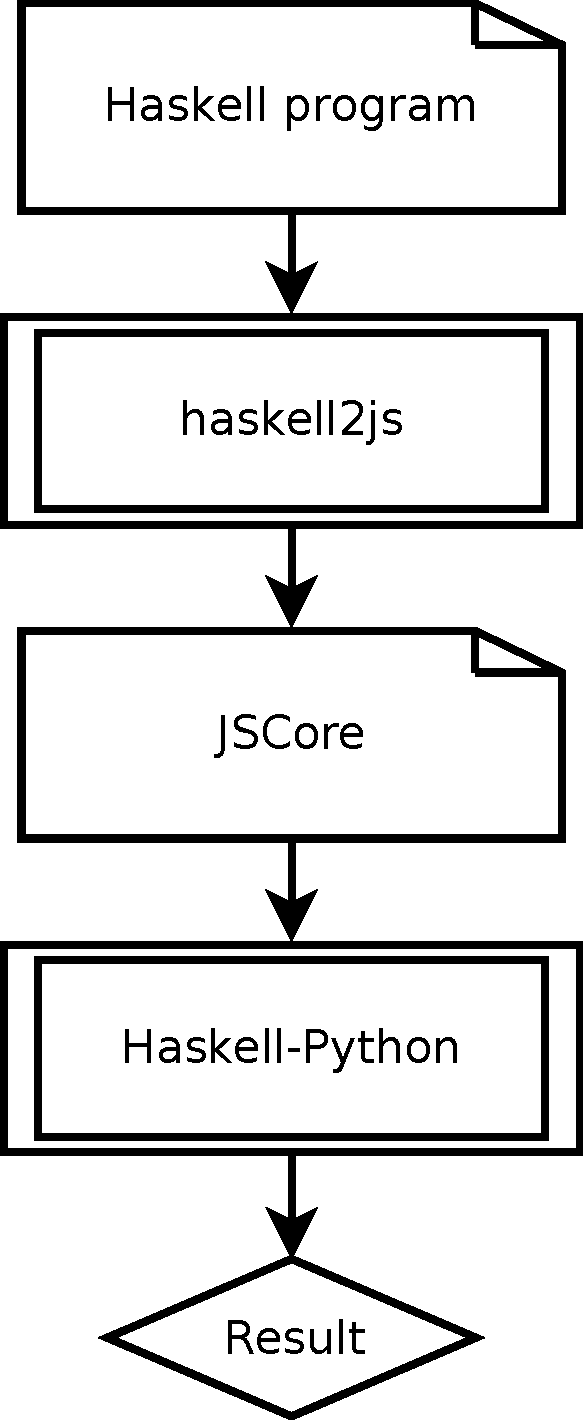
\includegraphics[width=0.8\textwidth]{diags/pipe_w_haskell2js}
\caption{Pipeline with implementation of haskell2js using the GHC API}
\label{haskell2js}
\end{figure}

Very few of the initial plans regarding this project was actually realized in the implementation.
The GHC API was intended to be used to generate JSCore, but this failed do to a lack of experience
with Haskell and the GHC API (see figure \ref{haskell2js} for a description of the initially intended
pipeline). It was then discovered that a lot of the necessary code was already
written in GHC (the code that generates the external-core files), however, this code was not 
exported in any way. It was also deeply embedded in the GHC code. After several attempts at creating
the JSCore format, and some emails back and forth with the GHC team, these methods where abandoned.

The extcore package was then introduced, as it was thought to serve nicely for our purpose. This
does however add an extra step to the generation of JSCore, having to generate external-core
first. There is no way of working with external-core without parsing it from a file. See figure \ref{core2js}.

The reason for not using extcore from the beginning was that it was thought to not be very 
well supported, as the external-core format seems to be changing. This also turned out to be
the case. However, GHC also changes rapidly, and an implementation using the GHC API may not
work for very long either. A version linking to the GHC executable would most likely be the
worst choice.

A large amount of time was spent trying to generate this intermediate format.

The method described here worked well for very trivial Haskell programs, however, it turned out that
the extcore package was not able to parse any nontrivial external-core files generated by GHC versions later 
than 6.10.

